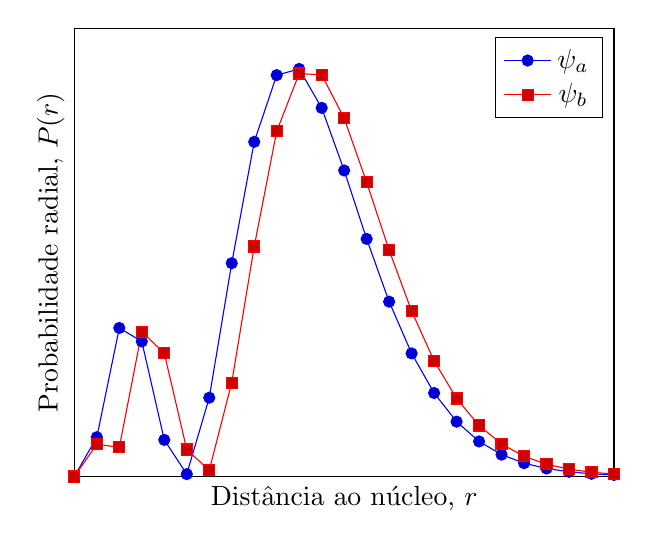
\begin{tikzpicture}
    \begin{axis}
    [
        xlabel={Distância ao núcleo, $r$},
        ylabel={Probabilidade radial, $P(r)$},
        xmin=0,xmax=20,
        ymin=0,
        domain=0:20,
        ticks=none,
    ]
    \addplot 
        { x^2 * (1/22 * x * (4-x) * e^(-x/2))^2 };
    \addplot 
        { x^2 * (1/15.588 * (6 - 6 * x + x^2) * e^(-x/2))^2 };
    \node at (1,0.1)    
        {$\psi_a$};
    \node at (9,0.1) 
        {$\psi_b$};
    \legend{$\psi_a$,$\psi_b$}
    \end{axis}
\end{tikzpicture}